\newpage
\section{Solution construction}\label{sec:solution-construction}

This section describes the process of how to transform or decode an individual.
This transformation aims to create a solution to the painting placement problem,
which is a sequence of placement points for the paintings.
There are multiple steps to this process.

\begin{enumerate}
    \item Individual decoding (\ref{subsec:individual-decoding}).
    \item Slicing tree construction (\ref{subsec:slicing-tree-construction}).
    \item Slicing layout construction (\ref{subsec:slicing-tree-construction}).
    \item Using placement heuristic to create a painting placement solution (\ref{subsec:placement-heuristic}).
\end{enumerate}

Steps in the transformation of an individual to the painting placement solution are
in figure~\ref{fig:layout-construction-steps}.
All of these steps are explained in the following text.


\begin{figure}[h!]
    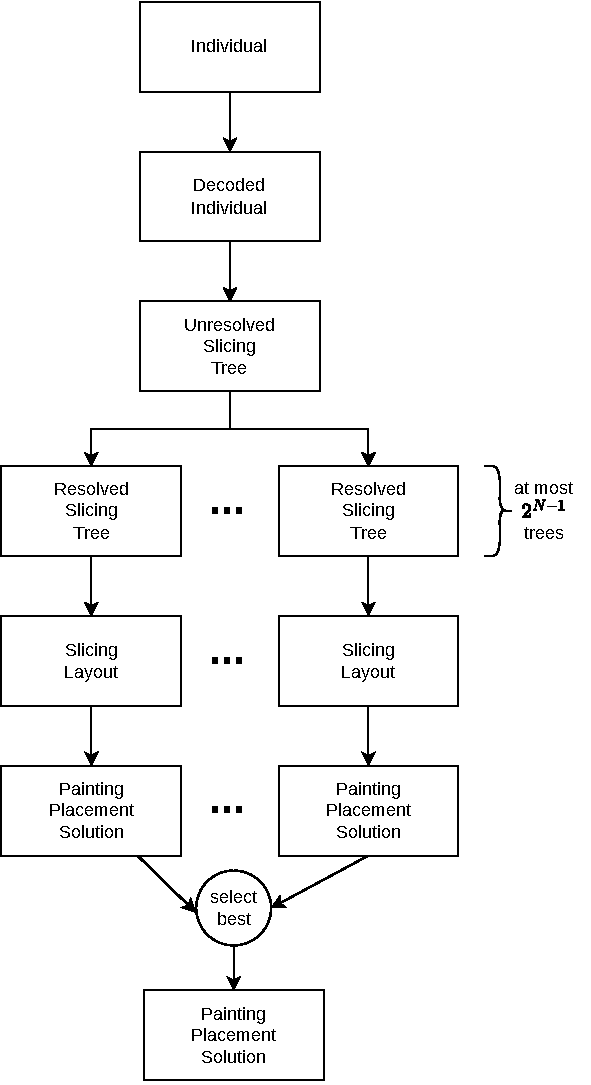
\includegraphics[height=0.65\textheight, center]{layout_construction_steps}
    \caption[Transformation of an individual to the painting placement solution]
    {Steps in the transformation of an individual to the painting placement solution.}
    \label{fig:layout-construction-steps}
\end{figure}

\subsection{Individual decoding}\label{subsec:individual-decoding}
First, we must decode an individual to the representation from which a slicing layout can be constructed.
A decoded individual is composed of painting sequence, slicing order, and orientations.
An example of individual decoding is in figure~\ref{fig:individual-decoding}.

Let us use the notation for painting sequence as $PS$, slicing order as $SO$, and orientations as $OR$.
$PS$ contains painting identifiers, $SO$ contains information used to construct slicing layout,
and $OR$ contains type of the cuts.\\

\navesti{Cut type} in $OR$  can take up three values.
\begin{itemize}
    \item $H$ for horizontal.
    \item $V$ for vertical.
    \item $*$ for wildcard, that can take up any value $H$ or $V$.
\end{itemize}

The introduction of the wildcard cut type $*$ is a novel idea proposed in this thesis.
In literature, only $H$ and $V$ cut types are used~\cite{friedrichIntegratedSlicingTree2018, changSlicingTreeRepresentation2013, liuMultiimprovedGeneticAlgorithm2012, hwangGeneticAlgorithmApproach2009}.

\subsubsection*{Decoding random keys}

Decoding $PS_{rk}$ to $PS$ and $SO_{rk}$ to $SO$ is the same as the RKGA in~\cite{beanGeneticAlgorithmsRandom1994}.
The graphical illustration is in figure~\ref{fig:individual-decoding} marked as~\textit{random key decoder}.
Decoding random keys in $PS_{rk}$ and  $SO_{rk}$ can be explained in the following steps on a sequence of four numbers $S = 0.3, 0.2, 0.4, 0.1$\,.

\begin{enumerate}
    \item Create $S'$ by adding a lower index to each element from $S$, which marks its ordinal position starting from one.
    $S' = 0.3_1, 0.2_2, 0.4_3, 0.1_4$\,.
    \item Sort $S'$ in descending order. $S' = 0.1_4, 0.2_2,  0.3_1, 0.4_3$\,.
    \item Take lower indexes of $S'$.
    It is the result – $4, 2, 1, 3$.
\end{enumerate}


\subsubsection*{Orientation probabilities decoding}

Last part of the individual, matrix $OR_{prob} \in \real^{N-1, 3}$, decodes to $OR$, which is a sequence of cut types.
The graphical illustration is in figure~\ref{fig:individual-decoding} marked as~\textit{orientation decoder}.

Decoding $OR_{prob}$ to $OR$ translates each row to one cut type.
Thus, decoding orientation probabilities can be explained for one row, say $R = 0.7, 0.2, 0.1$
in the following steps.


\begin{enumerate}
    \item Create $R'$ by adding lower index $H$ to the first, $V$ to the second, and $*$ to the last $R$'s elements.
    $R' = 0.7_H, 0.2_V, 0.1_*$
    \item Select element from $R'$ with the maximum value. $\max R' = 0.7_H$.
    \item Take lower index of $\max R'$.
    It is the result – $H$.
\end{enumerate}

There is one exception to the steps described above.
It is the limit on the maximum number of $*$ cut types produced by $OR_{prob}$ decoding.
Let us call this limit $k$.
If the limit is not applicable, i.e., $k \geq N-1$, there is no change to decoding steps 1--3 described above.
However, only the first $k$ wildcard cut types $*$ with the highest value are considered if applicable.
It is achieved by setting the value to $0$ (only for the duration of the decoding) to the bottom $N-1-k$ wildcard cut types $*$ with the lowest values.
Then the same 1--3 decoding steps are applied as described above.

One example where the limit on wildcard cut types $*$ applies is for the $k=1$ and $OR_{prob}$ that has two rows, $R_1 = 0.2, 0.3, 0.5$ and $R_2 = 0.1, 0.2, 0.7$.
Without exception, the result is $*, *$.
However, considering the exception on the maximum limit $k=1$, the result is $V, *$.
Reason is that in $R_2$, wildcard $*$ has value $0.7$,
which is higher than value of $*$ in $R_1$, which is $0.5$.

\begin{figure}[h!]
    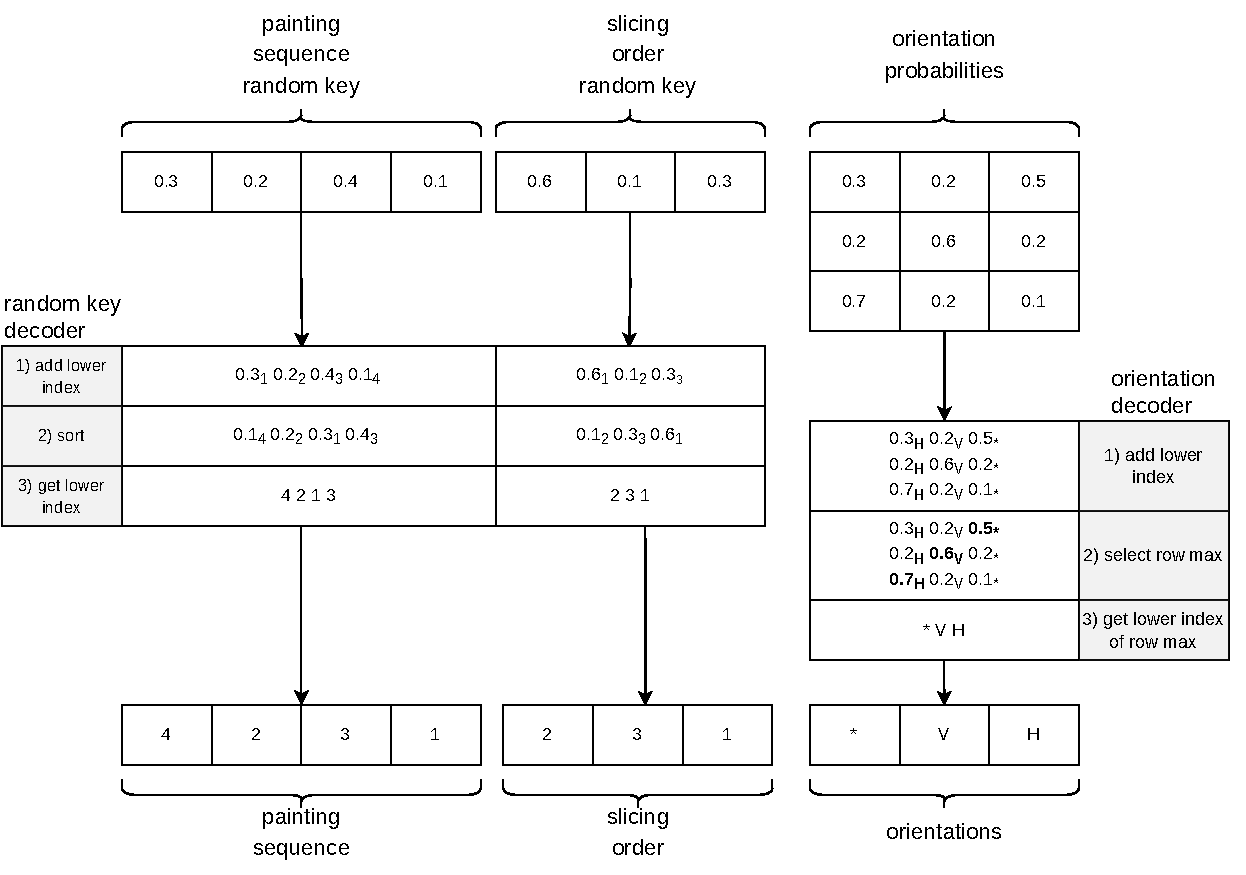
\includegraphics[width=1.1\textwidth, left]{individual_decoding}
    \caption[Individual decoding example]{
        Individual decoding example. Both the painting sequence random key and slicing order random key
        are decoded using the same procedure.
        The decoded individual is used to construct an unresolved slicing tree. }
    \label{fig:individual-decoding}
\end{figure}

\subsection{Slicing layout construction}\label{subsec:slicing-tree-construction}
In the previous subsection, decoding an individual is described.
The decoded individual consists of three parts – painting sequence, slicing order, and orientations.
From this representation, a slicing layout can be constructed.\\

\navesti{Slicing layout} is the recursive partitioning of space to rectangles using horizontal and vertical cuts.\\

Construction of the slicing layout from painting sequence, slicing order, and orientations has three steps, which are as follows.

\begin{enumerate}
    \item Construct an unresolved slicing tree from a decoded individual.
    \item Resolve an unresolved slicing tree.
    \item Create a slicing layout using a resolved slicing tree.
\end{enumerate}

\subsubsection*{Slicing tree construction}

First, let us describe what a slicing tree is.
The slicing tree was first introduced in 1982 by Otten~\cite{ottenAutomaticFloorplanDesign1982} to solve automatic floorplan design.
In the most general sense, it is a tree that codes the recursive division of space into rectangles using horizontal and vertical cuts.
A slicing tree can thus be used to construct a slicing layout.
According to~\cite{laiSlicingTreeComplete2001}, a slicing tree is a complete representation of a slicing layout.
That means every possible slicing layout has at least one slicing tree representing it.
This thesis defines and uses the slicing tree in two variants.\\

\navesti{Resolved slicing tree} is a binary tree with internal nodes having values from $\{H, V\}$
and leafs having values from the painting sequence.\\

\navesti{Unresolved slicing tree} is an extension of a resolved slicing tree where internal nodes have values from $\{H, V, *\}$. \\

Cut types $H$ for horizontal and $V$ for vertical are common for both types of the slicing tree.
An unresolved slicing tree can also contain the wildcard cut type $*$.

Next, we can use a decoded individual to construct an unresolved slicing tree.
This construction is graphically illustrated in the left part of a figure~\ref{fig:slicing-tree-construction}.
During this process, the painting sequence results in leaf nodes, slicing order determines the shape of a tree, and orientations are the values assigned to internal nodes.
Thus, each decoded individual represents one unresolved slicing tree.

Finally, an unresolved slicing tree is resolved.
Resolving is graphically illustrated in the right part of a figure~\ref{fig:slicing-tree-construction},
where the unresolved tree contains one wildcard symbol $*$ as a root.
By resolving this tree, $*$ is first replaced by $H$ and then by $V$.
In this case, resolving the unresolved slicing tree produces two resolved slicing trees,
which differ in root node value.
In the general case, an unresolved slicing tree can at most resolve to $2^k$ resolved slicing trees,
where $k$ is the number of internal nodes, i.e., the nodes that can contain wildcard $*$.
Reformulation for a decoded individual is that decoded individual can, at most, represent
$2^k$ resolved slicing trees, where $k$ is the number of orientations.



\subsubsection*{Slicing layout}

Next, we can construct a slicing layout using a resolved slicing tree.
Input to the construction has three parts that are as follows.

\begin{enumerate}
    \item Layout to partition.
    \item Areas of paintings to place.
    \item Resolved slicing tree
\end{enumerate}

The layout is the wall on which the paintings are placed.
Areas of the paintings are retrieved using the resolved slicing tree,
which contains painting identifiers as leaf nodes.

Construction can be described using figure~\ref{fig:slicing-layout-dimensions}.
On the left is an input to the construction – three paintings $1,2,3$ with areas $a_1, a_2, a_3$ and resolved slicing tree.
Then, we recursively traverse the resolved slicing tree.
Depending on the node value, there are three possible actions.

\begin{itemize}
    \item $H$ – cut layout horizontally.
    \item $V$ – cut layout vertically.
    \item Otherwise, assign node value to the layout.
\end{itemize}

After performing the cut, the process mentioned above is recursively repeated
for the left and right child.
If the cut is horizontal, the left child is given the upper part of the cut as its layout, and the right child is given the lower part.
If the cut is vertical, the left child is given the left part of the cut as its layout, and the right child is given the right part.
It can be seen in the middle part of the figure, where the cut is vertical.
The left child is an orphan, i.e., it has no children.
Thus, the left part of the cut is assigned value 1.
The right child is not an orphan, meaning the process is applied recursively to the right part of the cut and the right child.
It is depicted on the right part of the figure.

The last part of creating a slicing layout is the position of the cut.
As mentioned above, the resolved slicing tree has horizontal and vertical cut types.
Each cut type's position is determined proportionally to the area of rectangles assigned to the cut result.
Again, it can be described using an example in figure~\ref{fig:slicing-layout-dimensions}.
The first cut is vertical, where the left part of the cut is assigned rectangles $1$ and the right part is assigned rectangles $2,3$.
The vertical cut thus splits the layout into two parts – the left part having $1/3$ of the total layout area and the right part
having the rest.

\afterpage{%
    \clearpage% Flush earlier floats (otherwise order might not be correct)
    \begin{landscape}% Landscape page
        \begin{figure}[]
            \centering
            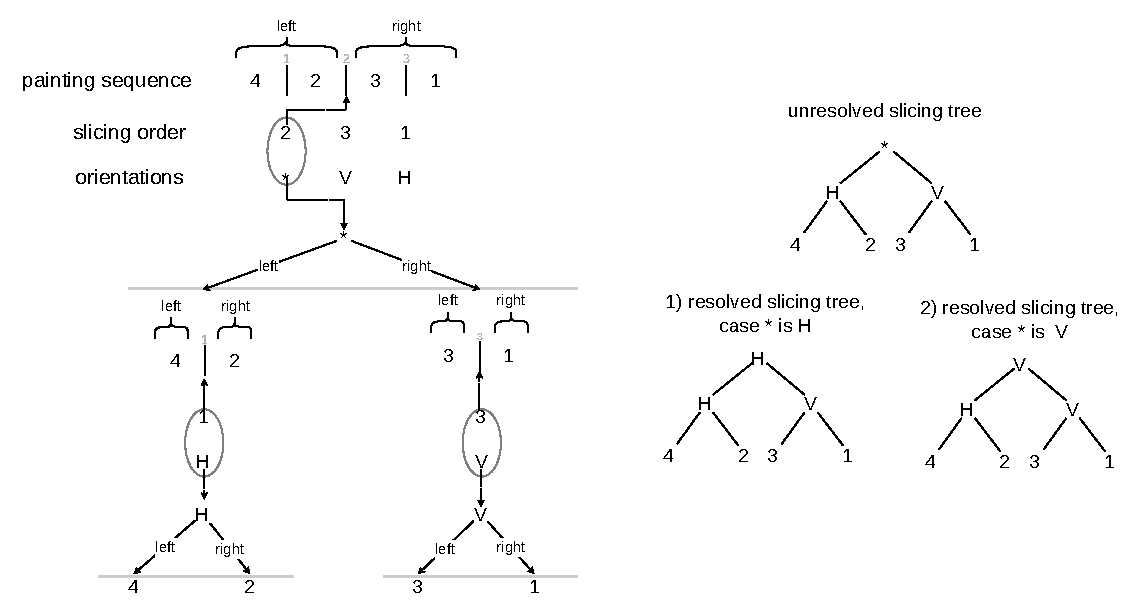
\includegraphics[width=1.5\textwidth]{slicing_tree_construction}
            \caption[Slicing tree construction]{
                On the left is an example of unresolved slicing tree construction from a decoded individual.
                On the right is an example of resolving an unresolved slicing tree.}
            \label{fig:slicing-tree-construction}
        \end{figure}
    \end{landscape}
    \clearpage% Flush page
}

\afterpage{%
    \clearpage% Flush earlier floats (otherwise order might not be correct)
    \begin{landscape}% Landscape page
        \begin{figure}
            \centering
            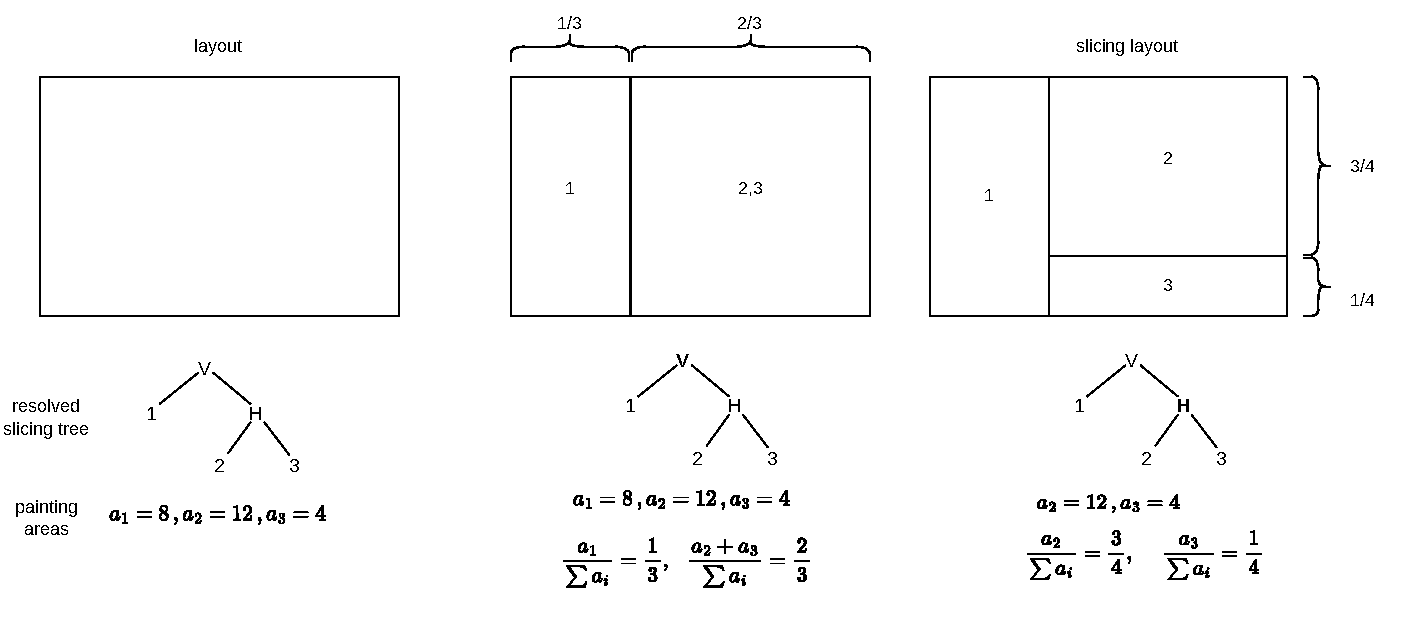
\includegraphics[width=1.5\textwidth]{slicing_layout_dimensions}
            \caption[Slicing layout construction]
            {Example of a slicing layout construction from a resolved slicing tree, painting areas, and layout. There are three paintings, $1,2,3$ together with their areas $a_1, a_2, a_3$.
            The position of a cut is determined proportionally to the area of the paintings.} \label{fig:slicing-layout-dimensions}
        \end{figure}
    \end{landscape}
    \clearpage% Flush page
}


\newpage

\subsection{Placement heuristic}\label{subsec:placement-heuristic}

The placement heuristic is the last part of transforming an individual into a painting placement solution.
Input to the heuristic is the slicing layout together with paintings, and output is the painting placement solution.
The pseudocode of the proposed placing heuristic is in algorithm~\ref{alg:placement-heurictic}.

\begin{algorithm}[H]
    \SetAlgoLined
    \LinesNumbered

    \SetKwData{PlacedPaintings}{placedPaintings}
    \SetKwData{Painting}{painting}
    \SetKwData{PlacedPainting}{candidate}
    \SetKwData{Paintings}{paintings}
    \SetKwData{Best}{best}
    \SetKwData{SlicingLayout}{slicing layout}
    \SetKwData{Nil}{NIL}
    \SetKwData{EmptyList}{EMPTY LIST}

    \SetKwFunction{PossiblePlacementPoints}{possiblePlacementPoints}
    \SetKwFunction{Place}{place}
    \SetKwFunction{Objective}{objective}

    \SetKw{In}{in}
    \SetKw{Or}{or}


    \KwData{\SlicingLayout, \Paintings}
    \KwResult{painting placement solution} \BlankLine

    %%%%%%%%%%%%%%%%%%%%%%%%

    \PlacedPaintings $\leftarrow$ \EmptyList \\

    \For{$painting$ \In \Paintings} {
        \Best $\leftarrow$ \Nil \\
        \For{$point$ \In \PossiblePlacementPoints{painting, \PlacedPaintings, \SlicingLayout}} {
            \PlacedPainting $\leftarrow$ \Place{painting, point}\\
            \If{\Best == \Nil\\
            \Or \Objective{\PlacedPaintings$+$\PlacedPainting, \SlicingLayout}\\
                $<$  \Objective{\PlacedPaintings $+$ \Best, \SlicingLayout}}{
                \Best $\leftarrow$ \PlacedPainting
            }
        }
        \PlacedPaintings += \Best
    }

    \KwRet{\PlacedPaintings}

    \caption{Placement heuristic}\label{alg:placement-heurictic}
\end{algorithm}

The proposed heuristic is greedy and iterative.
Iterative means that it creates the painting placement solution gradually, as it
tries to place one painting after another using the slicing layout.
It is greedy because, at each iterative step, it places a painting in a way that minimizes the objective value.

As mentioned earlier, the slicing layout recursively divides space into rectangles.
Additionally, each rectangle in the slicing layout has been assigned a painting identifier.
The function in algorithm~\ref{alg:placement-heurictic} \verb|possiblePlacementPoints|
uses this assigned space as an allocated area.\\

\navesti{Allocated area} for a painting is a rectangle from a slicing layout to which its identifier is assigned.\\

It means that every slicing layout has one allocated area for each painting.
Also, the allocated area does not necessarily need larger dimensions than the painting.
E.g., the width of a painting might be greater than the width of its allocated area.
An example of a painting and its allocated area is in figure~\ref{fig:allocated-area}.

An important part of the algorithm~\ref{alg:placement-heurictic}
is function \verb|possiblePlacementPoints| on line 4.
This function returns points that the heuristic tries for placing a painting.
Implementation in this thesis is called the corner-placing heuristic.\\

\navesti{Corner-placing heuristic} is a placing heuristic that considers four painting placement points for each painting
– the allocated area's bottom-left, bottom-right, top-left, and top-right corners.\\

Examples of the painting placement points created by the corner-placing heuristic are in figure~\ref{fig:allocated-area}.
On the left, we can see that the allocated area's dimensions are sufficient
to try all four points.
In the middle, there are only two points where the placing of a painting does not
result in it being outside the allocated area.
On the right, all points result in being outside the allocated area.
Additionally, figure~\ref {fig:corner-placing-heuristic} shows iteration of the corner-placing heuristic considering one placement point.

\begin{figure}[h!]
    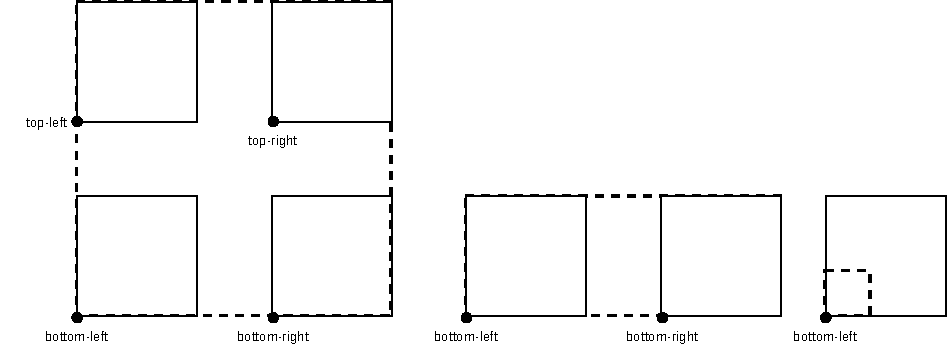
\includegraphics[width=1.2\textwidth, center]{allocated_area}
    \caption[Examples of the painting placement points created by the corner-placing heuristic]
    {Examples of the painting placement points created by the corner-placing heuristic
    for three different allocated areas that are plotted using a dashed line.}
    \label{fig:allocated-area}
\end{figure}

\begin{figure}[h!]
    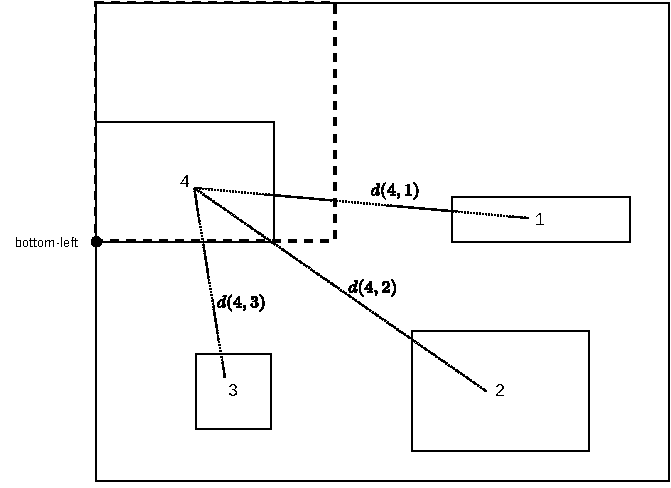
\includegraphics[width=0.8\textwidth, center]{corner_placing_heuristic}
    \caption[Painting placement example]
    {Example of a painting 4 placed inside its allocated area using the corner-placing heuristic.
    The allocated area is plotted using a dashed line.
    Also, the distances between the placed painting and all other paintings are displayed using a dotted line.}
    \label{fig:corner-placing-heuristic}
\end{figure}
